% ---------------------------------------------------------------------------
\section{Simulations of the Solvable Model}
\label{sec:sims}

We now test the theory of \cref{sec:theory} in stochastic simulations of the toy model: first the predictions P1--P4, then the extensions of \cref{sec:general,sec:kernel,sec:remedy}, and finally robustness to the training setup.

\paragraph{Protocol.}
We simulate \cref{eq:model} with every source of finite-sample noise included. Each step draws a minibatch of problems, samples $K$ answers per problem, takes the majority vote, and applies the SGD step of \cref{sec:theory}.
Unless stated otherwise we use REINFORCE with $K{=}3$ and train until every problem has left the unstable window.
Initial preferences are exactly balanced, the shared parameter starts at $v{=}0$, and the initial majority is correct for $80\%$ of problems, so collapse can only be driven by sampling noise.
We call a run collapsed when the order parameter $\Phi=|\langle\mathrm{sign}\,z_i\rangle|$, which is $0$ for balanced answers and $1$ when all problems give the same answer, exceeds $0.5$ at the end of training. $N_c$ is the midpoint of a logistic fit of $P(\text{collapse})$ against $\ln N$.
All settings are listed in \cref{app:details}, and code and raw results are available at \url{https://github.com/pd2714/RLVR_instability}.

\begin{figure*}[t]
\centering
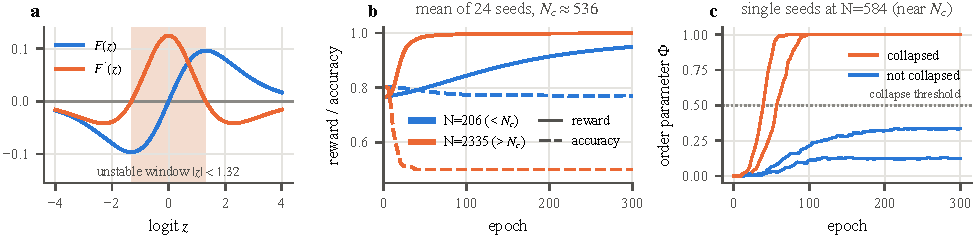
\includegraphics[width=\textwidth]{../figures/fig_mechanism.pdf}
\caption{\textbf{Mechanism.} (a)~Single-problem drift $F$ and its slope $F'$. The shaded window $|z|<z^\star$ is where a shared push is amplified. (b)~Majority-vote reward (solid) and accuracy against the hidden labels (dashed) at $\lambda{=}0.1$, $a{=}0.5$, averaged over 24 seeds. The two runs differ only in the number of training problems, which lies below (blue) or above (orange) the fitted $N_c\approx536$. Below $N_c$, local sharpening wins: the reward rises and accuracy stays near its initial level. Above $N_c$, the reward rises \emph{faster} and accuracy falls to chance, because every problem converges to the same answer. (c)~Order parameter $\Phi$ of four individual seeds with identical settings at $N=584$, the simulated size closest to $N_c$. Orange runs end above the collapse threshold $\Phi=0.5$ (dotted) and blue runs below it. Sampling noise decides the outcome within the first ${\sim}100$ epochs, while problems are still inside the unstable window, and $\Phi$ then freezes. A run can also collapse partially (upper blue curve).}
\label{fig:mechanism}
\end{figure*}

\subsection{A sharp transition at a single critical amplification (P1--P4)}
We begin with the basic phenomenon (P1): whether a sharp transition in $N$ appears without being built into the model.
Above a threshold number of problems, the self-assessed reward goes to one while accuracy falls to chance, because every problem converges to the same answer (\cref{fig:mechanism}b).
Below it, the same algorithm with the same hyperparameters only sharpens each problem.
Near $N_c$, runs with identical settings differ only in their sampling noise, and some collapse while others do not (\cref{fig:mechanism}c).
The outcome is decided early, while problems are still inside the unstable window, and does not change afterwards.
The probability of collapse rises from $0$ to $1$ within a factor of a few in $N$ (\cref{fig:scaling}a).

\begin{figure*}[t]
\centering
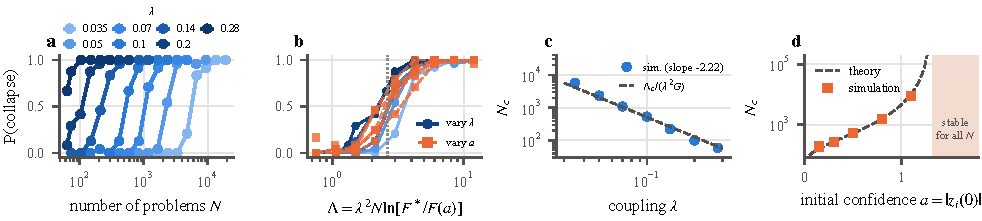
\includegraphics[width=\textwidth]{../figures/fig_scaling.pdf}
\caption{\textbf{Critical number of problems.} (a)~Probability of collapse against $N$ for seven coupling strengths ($a{=}0.5$). (b)~The same data, together with a sweep over initial confidence $a$ (orange, $\lambda{=}0.1$), plotted against the predicted amplification $\Lambda=\lambda^2N\ln[F^\star/F(a)]$. Curves spanning a $64\times$ range in $\lambda^{-2}$ and critical sizes from $60$ to $8740$ collapse onto a single transition at $\Lambda_c\approx2.6$ (dotted). (c)~$N_c$ against $\lambda$. The fitted slope is $-2.22$, compared with the predicted $-2$ plus a logarithmic correction. (d)~$N_c$ against initial confidence. The dashed line is the theory with the single constant $\Lambda_c$. Beyond $z^\star$ (shaded) the theory predicts no collapse at any $N$.}
\label{fig:scaling}
\end{figure*}

Having established the transition, we next ask where it occurs (P2). \Cref{eq:Nc} predicts that the coupling $\lambda$ and the initial confidence $a$ enter only through the amplification $\Lambda$.
Varying the coupling moves $N_c$ by two orders of magnitude, with $N_c\propto\lambda^{-2.2}$ (\cref{fig:scaling}c). The small excess over $-2$ is the predicted $\ln(1/\delta)$ correction, since the noise seed scales with $\lambda$ (\cref{app:seed}).
Varying the initial confidence moves $N_c$ as $1/\ln[F^\star/F(a)]$ (\cref{fig:scaling}d).
Plotted against $\Lambda$, all sweeps collapse onto a single transition at $\Lambda_c\approx2.6$ (\cref{fig:scaling}b), and this one constant then predicts $N_c$ for every other configuration below.
Fitted values are in \cref{app:fits}, and \cref{app:mfcheck} checks the form of \cref{eq:Nc} exactly in the noise-free limit.

The last two predictions also hold.
Batch size changes $N_c$ only logarithmically, and not at all under the linear scaling rule $\eta\propto B$ (P3, \cref{app:batch}).
Confident models ($a>z^\star$) never collapse, even far beyond the threshold for uncertain models and under much longer training: not a single problem flips its answer (P4, \cref{app:stable}).

\subsection{Heterogeneity, feature coupling and a remedy}
\label{sec:hetero}
The sweeps above use a homogeneous population with no coupling besides the shared direction. We now test heterogeneous confidence (\cref{sec:general}), prediction-aligned feature coupling (\cref{sec:kernel}) and the marginal-entropy remedy (\cref{sec:remedy}). Details are in \cref{app:hetero}.

Real models are uncertain on some problems and confident on others.
For seven distributions of initial confidence, the amplification $\lambda^2NG[\rho_0]$, computed from the initial distribution alone, locates the transition in every case, with the same $\Lambda_c$ (\cref{fig:hetero}a).
What matters is the sign of the instability index $\langle F'\rangle$, not the mean confidence. A population that is mostly confident still collapses, only at a much larger $N$, as long as some problems start inside the window. A population with $\langle F'\rangle<0$ from the start never collapses.

Heterogeneity changes $G$ but leaves the coupling between problems unchanged. We next add the protective coupling predicted by the kernel theory: a coupling aligned with each problem's initial preference, so that sharpening one problem also sharpens the others, as happens when a network generalizes.
The kernel theory (\cref{eq:kernel}) predicts that $N_c$ grows with the strength $\mu$ of this coupling and diverges at a finite $\mu_c$.
Simulations agree (\cref{fig:hetero}b): $N_c$ grows with $\mu$, and beyond $\mu_c$ no run collapses at any $N$ we tested.
When sharpening is shared strongly enough across problems, adding data no longer leads to collapse.

Finally, the marginal-entropy bonus of \cref{sec:remedy} prevents collapse above the predicted threshold $\beta_c\approx\tfrac12$ (\cref{eq:beta}, \cref{fig:hetero}c).
Above it, no run collapses at any $N$ we tested, and because the bonus does not slow per-problem sharpening, accuracy stays at its sharpening-only value.

\begin{figure*}[t]
\centering
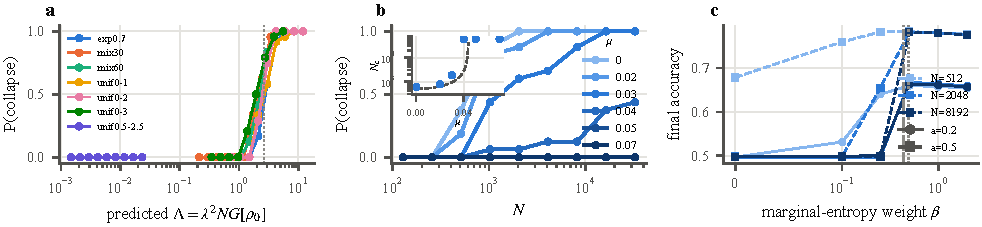
\includegraphics[width=\textwidth]{../figures/fig_hetero_feature_remedy.pdf}
\caption{\textbf{Generalizations.} (a)~Heterogeneous initial confidence. $P(\text{collapse})$ against the amplification $\lambda^2NG[\rho_0]$ predicted from the initial distribution alone; the dotted line is $\Lambda_c$ from \cref{fig:scaling}. (b)~Prediction-aligned coupling $\mu$ delays and then eliminates collapse. Inset: $N_c$ against $\mu$ with the prediction $1/(\lambda^2G/\Lambda_c-\mu^2)$. Points at the top edge did not collapse. (c)~Final accuracy with the marginal-entropy bonus. Vertical lines mark the predicted $\beta_c(a)$.}
\label{fig:hetero}
\end{figure*}

\subsection{Robustness to the training setup}
All runs above use REINFORCE with $K=3$, binary answers and plain SGD. Varying each of these choices leaves the law intact (\cref{sec:robust}).
GRPO collapses at the same $N_c$ as REINFORCE, as predicted for $K=3$ (\cref{sec:single}). Larger groups raise $N_c$ in the order predicted by $G_K$, many-answer policies collapse at a similar $\Lambda_c$, and Adam keeps $N_c\propto\lambda^{-2}$ with a larger constant (\cref{fig:robust}).

\begin{figure*}[t]
\centering
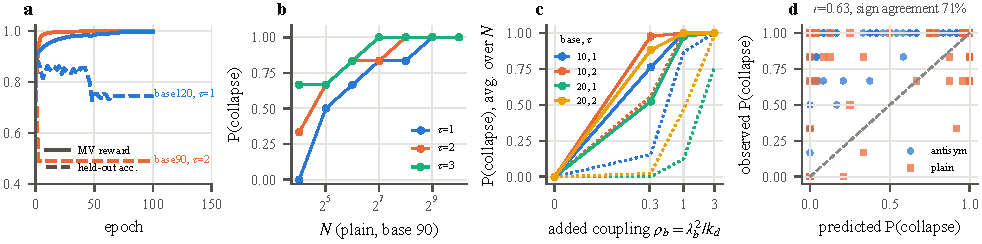
\includegraphics[width=\textwidth]{../figures/fig_nn.pdf}
\caption{\textbf{Label-free RL on a small Transformer.}
(a)~Majority-vote reward (solid) and held-out accuracy (dashed) of one run at $N{=}512$, for base 90 at $\tau{=}2$ (orange) and base 120 at $\tau{=}1$ (blue).
(b)~Plain Transformer, base 90: probability of collapse against $N$ at three temperatures, as the observed fraction of 6 seeds.
(c)~Antisymmetric Transformer: probability of collapse, averaged over $N$, against the added shared coupling $\rho_b$, for each base and $\tau$. Solid: observed. Dotted: kernel-calibrated surrogate in the same color, from 24 simulated seeds per point. $\rho_b{=}0$ is drawn at the left edge.
(d)~Observed against surrogate-predicted probability of collapse. Each point is one condition at one training-set size $N$, summarizing 6 RL runs, so observed values are fractions of 6 and many points overlap. Dashed: perfect calibration; points above it collapse more often than predicted. Title: Pearson correlation $r$ and the fraction of points in which prediction and observation lie on the same side of $\tfrac12$.}
\label{fig:nn}
\end{figure*}

% ---------------------------------------------------------------------------
\section{A Small Transformer Trained Without Labels}
\label{sec:nn}

\Cref{sec:sims,sec:robust} test the theory on the toy model, where the coupling is known exactly. A real network has many shared directions, and its coupling must be measured.
We therefore ask whether quantities measured on an initial \emph{network}, before any RL step, predict whether label-free RL collapses.
We describe the task and models, form predictions from the initial network, and then compare them with the outcomes of RL.

\subsection{Setup}
\label{sec:nnsetup}

\paragraph{Task and architectures.}
Inputs are six digits, and the answer is $+$ if $x_1+x_2+x_3>x_4+x_5+x_6$ and $-$ otherwise.
The policy is a small Transformer that reads out an answer logit $z(x)$ from a classification (CLS) token (architecture in \cref{app:details}). Answers are sampled at temperature $\tau$, so the logit of \cref{sec:single} is $z/\tau$.
Raising $\tau$ makes the same network less confident, which moves problems into the unstable window and increases $G$, without changing the kernel ratios (every kernel entry scales as $1/\tau^2$). We therefore use $\tau$ to vary the entropy of the base model.
To mimic a pretrained base model with partial competence, we first train briefly with labels. ``Base $n$'' denotes the model after $n$ supervised steps.

We describe the coupling of each network by the kernel ratios of \cref{sec:kernel}: $k_u/k_d'$ measures the shared coupling, which drives collapse, and $k_s/k_d'$ the prediction-aligned coupling, which protects against it. We measure them on the initial network, from per-example gradients on a sample of unlabeled problems.
We study two architectures chosen to sit at opposite ends of \cref{eq:kernel}: one whose shared coupling far exceeds its protective coupling, and one with essentially no shared coupling but strong protection. Together they test the kernel prediction at both extremes, and the second provides a clean baseline into which a controlled shared coupling can be added back.
Let $h(x)$ denote the network's readout, the logit difference computed from the CLS token. The \emph{plain} model uses it directly, $z(x)=h(x)$. Its readout features share a large input-independent component, so its shared coupling is an order of magnitude larger than its protective one.
The \emph{antisymmetric} model uses the same network and parameters but constrains its logit to be antisymmetric under exchanging the two halves of the input, like an odd function: $z(\bar x)=-z(x)$, where $\bar x=(x_4,x_5,x_6,x_1,x_2,x_3)$. We impose this by running the network on both inputs and taking the difference, $z(x)=h(x)-h(\bar x)$. The constraint matches the task, since exchanging the halves always flips the correct answer. It also removes the shared direction: a parameter change that shifts $h$ by the same amount on every input, which in the plain model pushes all problems toward the same answer, cancels in the difference. This leaves essentially no shared coupling while keeping a strong protective one.
For each architecture we use two base models (\cref{tab:conditions}).

In the antisymmetric model we reintroduce a controlled shared coupling through a scaled output bias, $z\mathrel{+}=\lambda_bb$. This adds $\lambda_b^2$ to $k_u$ and leaves $k_s$ and $k_d'$ essentially unchanged.
We measure the dose by $\rho_b=\lambda_b^2/k_d$, relative to the self-kernel $k_d$ of the bias-free model.

\paragraph{RL runs and parameter-free predictions.}
We run label-free majority-vote RL (REINFORCE, $K{=}3$, plain SGD) on the first $N$ problems of an unlabeled pool, with the step scaled so that each visit moves a problem's own logit by the same amount as in the toy model.
We call each combination of architecture, base model, temperature and dose a \emph{condition}, and run each condition at seven training-set sizes with six seeds (\cref{app:nndetails}).

From the initial network alone, we then predict whether training collapses.
Our main predictor is a \emph{kernel-calibrated surrogate}: the stochastic toy model of \cref{sec:sims} with $\lambda^2=k_u/k_d'$, $\mu^2=k_s/k_d'$, the network's own initial logits, and the same training settings.
As simpler baselines we use the bare threshold $\Lambda(N)>\Lambda_c$ of \cref{eq:kernel}, with $\Lambda_c$ from the toy model, and a deterministic mean-field version of the kernel dynamics (\cref{app:kernel}).
None of these predictors is fitted to the network's RL outcomes.

\subsection{Results}
\label{sec:nnresults}

\paragraph{Collapse and what controls it.}
Label-free RL reproduces the failure seen in language models (\cref{fig:nn}a). In collapsing runs the majority-vote reward goes to one while training \emph{and held-out} accuracy fall to chance, because the network gives the same answer to every input.
Not every run fails this way: for the most confident plain model the reward also rises, but held-out accuracy stays far above chance.

The two architectures let us test whether this collapse requires a shared direction.
The antisymmetric network, which has none, \emph{never} collapses, as the surrogate predicts (\cref{fig:nn}c). This holds even for highly uncertain initializations, which would collapse at small $N$ given any appreciable shared coupling.
Adding a shared coupling back through the bias restores collapse in a dose-dependent way, and once it is comparable to the self-kernel ($\rho_b\ge1$) virtually every run collapses (\cref{fig:nn}c).
This is the network analogue of the $\lambda$-sweep of \cref{sec:sims}, and it directly tests the causal claim: the instability requires a direction that moves all answers together.

The plain network, which has a strong intrinsic shared direction, shows the two dependences reported for language models.
Its probability of collapse grows with $N$ (\cref{fig:nn}b), the small-set-stable, large-set-unstable pattern of \citet{he2026urlvr}, here at smaller $N$ because its shared coupling is much stronger than in our toy-model runs.
Raising the temperature, which increases the initial entropy, increases collapse monotonically for both base models (\cref{fig:nn}b, \cref{tab:conditions}).

\paragraph{Accuracy of the parameter-free predictions.}
We score each predictor on every condition and training-set size, counting agreement when the predicted and observed probabilities of collapse lie on the same side of $\tfrac12$.
The surrogate agrees in $71\%$ of cases (\cref{fig:nn}d), and more often far from threshold. The two simpler predictors do worse (\cref{app:nndetails}).
The errors are almost all in one direction: the real network collapses more often than its initial kernel predicts.
Most misses are antisymmetric networks with weak added coupling, which sit close to threshold, and confident plain networks at $\tau=1$, whose initial logits place almost no problems inside the unstable window.

The bias has a simple cause: the kernel changes during training, which breaks the fixed-kernel assumption of \cref{sec:kernel}. Feature learning quickly erodes the protective coupling, so the initial kernel underestimates the risk of collapse (\cref{app:kerneldrift}).

\paragraph{Marginal-entropy remedy.}
The bonus of \cref{sec:remedy} also prevents collapse in the network, but it does not rescue accuracy (\cref{fig:nnremedy}, \cref{app:nnremedy}).
The bonus penalizes only an imbalance of the pooled answers, so it damps only the uniform mode. The kernel has other collective modes that move many problems at once while keeping the answers balanced, and that are unrelated to the current predictions. \Cref{prop:instab} applies to each of them, so once the uniform mode is damped, the strongest of them takes over. The network still ends confident and balanced, but its answers follow a pattern set by its own features rather than by the task, and accuracy falls to chance.

